% Here we can discuss the Hardware components of the raspberry pi and why we chose such a device (GPU, GPIO, Bluetooth, WiFi, etc.)
In the early stages of development for our system, we prioritized the ability for fast prototyping over power efficiency. 
Since we pursued overpowered functionality for image processing, easy programmable GPIO pins, and wireless communication via Bluetooth and WiFi, our decision for a single board computer Raspberry Pi Model 3 was perfect.
Raspberry Pi Model 3's have been commonly known as amazing tools for creating projects extremely fast with its System On Chip (SOC) with a multi-core processor, GPU, I/O peripherals, Ethernet port, USB host, and so much more.
Using these Raspberry Pi's for sensor modules, we easily produced multiple sensors for communication with the database. 

\subsection{Background Setup Process} %I Hate this title
For ease of mass production and automation for sensor modules on our developmental side, we created shell scripts specifically for setup.
A key aspect of modifying our sensors was allowing secure shell (SSH) connection through pipeline via internet.
To properly install this framework into our sensor modules is by using:

\vspace{0.5cm}
\begin{lstlisting}[language=bash]
sudo apt-get install sshpass
\end{lstlisting}
\vspace{0.5cm}

One main component for easy debugging was the ability for direct connection with each individual sensor module through WiFi addressing.
Using SSH allows us to easily modify or test each individual sensor based off of their unique identifier.

Another installation needed to operate the Raspberry Pi's properly for our functionality is the GPIO pins.
Our sole purpose for GPIO programming is for the proximity sensors.
\vspace{0.5cm}
\begin{lstlisting}[language=bash]
sudo apt-get install python-dev python-rpi.gpio
\end{lstlisting}
\vspace{0.5cm}

% With 40 GPIO pins for each sensor module is obviously overkill, but allows room for expansion with features
By installing these two specific packages, we can fully implement the python library for GPIO operation.

The same setup script includes creating a local log folder containing all the files for occupy status, time stamps, and uuid.
Creating these files locally allows us to individually control and track information for each individual sensor independent from connection to the database.

The last part of the script initializes boot-up daemons to automatically run once the sensor is powered on.
\begin{lstlisting}[language=bash]
sudo cp ~/scripts/setup/sensor\_nodes/bootup\_ping\_script.sh /etc/init.d/
sudo update-rc.d /etc/init.d/bootup\_ping\_script.sh defaults
\end{lstlisting}
These two lines solely edit the initialization files so when the device is powered, it runs our boot-up script.
Once these files are implemented into the daemons, the sensor is able to be completely automated.
\subsection{Sensor Automation}
%%%%%%%%%%%%%%%%%%%%%%
\begin{figure}[ht!]
\centering
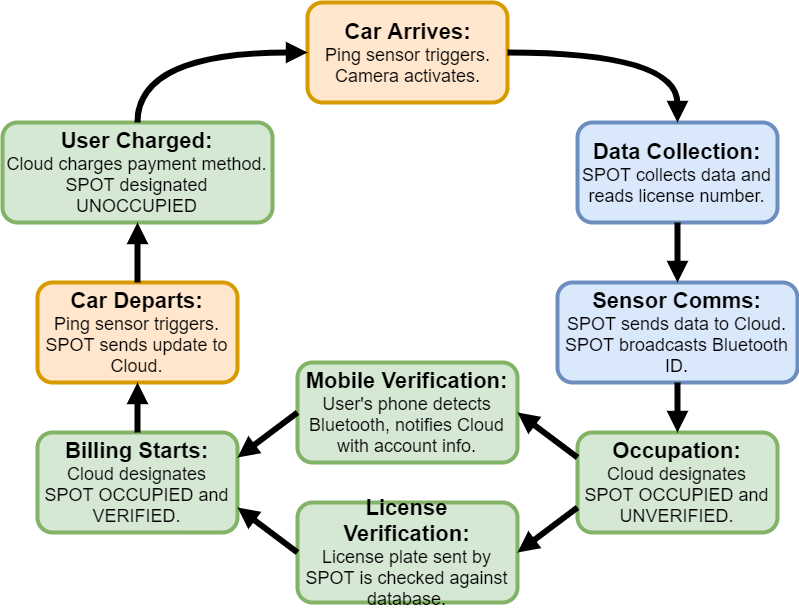
\includegraphics[width=0.7\textwidth]{pictures/EventFlowchart.png}
\caption{This demonstrates the flowchart that it continually repeating whenever a new car arrives at a SPOT.}
\end{figure}
%%%%%%%%%%%%%%%%%%%%%
For the convenience of administrative users, hardware operations are completely automated.
Using a Linux OS, we accomplished the automation through crontab. 
Crontab is a daemon that typically comes natively through Linux distributions. 
By editing the crontab file, we could schedule a single program to run periodically. 
However, we soon discovered this would not suffice because crontab had a minimum period of one minute and we needed to ping the spot at least every five seconds.
Periodically, we used a bash while loop to make a daemon that implements Linux calls like ‘sleep()’ to halt our program.
To send this process to the background we append ‘\&’ which commands a program to be thrown into the background. 
Altering these daemon background scripts allows our system to be initialized upon boot-up.
To avoid the program from throwing a signalling a close interrupt (SIGINT) error, our program is ran by ‘nohup’ which served to stop the program from throwing SIGINTS.
\begin{lstlisting}[language=bash]
nohup /pathto/program.sh \&
\end{lstlisting}

In our case we use:
\begin{lstlisting}[language=bash]
nohup  $\sim$/SPOT/scripts/setup/sensor\_nodes/background\_ping.sh \&
\end{lstlisting}

This was the specific file path and format for us to be able to run the background script.
In our file \textit{background\_ping.sh}, a series of scripts are called that automated the sensor module.
In the early stage of the script, we call python files that control GPIO peripherals for control over the proximity sensor.
After the python is executed for detecting if a car has approached the sensor module or not, a local status file is then written based from the results of the python. 
After the status is changed, we check to see if it is occupied or empty.
If the SPOT is occupied, we emit a red light and broadcast an eddystone beacon allowing the user to connect via our phone application. 
On the contrary, if the SPOT is vacant, a green light is emitted.
Once the status change is detected, the sensor uses a transfer script using a python function call to POST to the database with all the information needed for full functionality.

\subsection{Bluetooth Beacons}
%%%%%%%%%%%%%%%%%%%%%%
\begin{figure}[ht!]
\centering
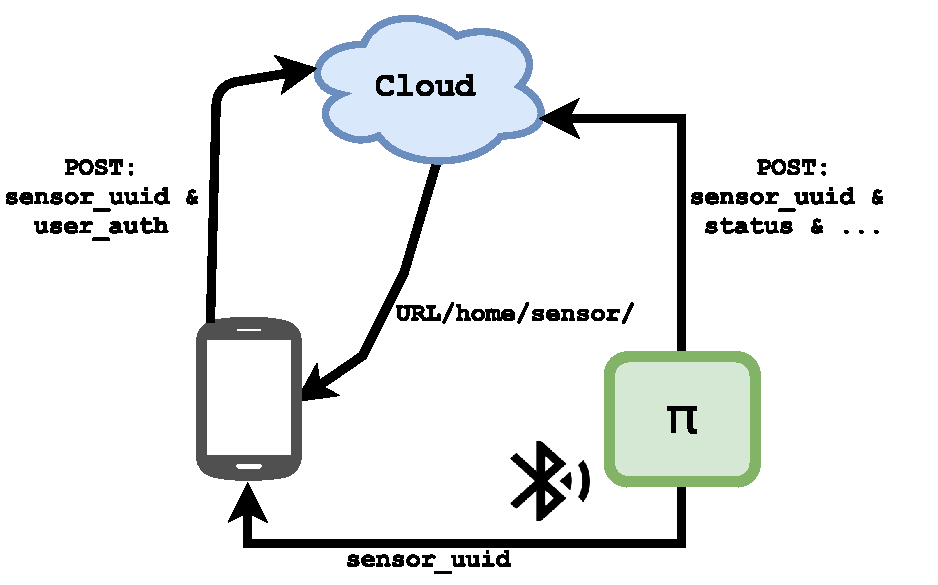
\includegraphics[width=0.85\textwidth]{pictures/BluetoothBeacon.pdf}
\caption{The process in which the user gets notified from the Bluetooth beacon, posts to the cloud their information, and gets redirected from the server.}
\end{figure}
%%%%%%%%%%%%%%%%%%%%%
Eddystone is a beacon format that can be used on both Android and iOS. 
Through the EddyStone Bluetooth Connection, we are able to format the payload in four different formats: UID, URL and TLM, EID. 
In the earlier stages of the project, we approached the broadcast as a simple URL using parameters to send specific information back and forth. 
This technique brings us a simple and direct way to link a URL with one or two parameters through Bluetooth. 
Unfortunately, this technique is extremely limited and the URL itself takes most of the bytes, while UID saves almost all the bytes for unique identification. 
The format each SPOT broadcasts is the UID format capable of broadcasting 20 bytes when activated.
With 20 bytes of being able to uniquely identify our sensor modules we have plenty of room for scalability. 
Using the phone application, we pick up the sensor's UID, tie it with the user account, then post to the cloud.

The UID payload has the following format:
\begin{center}
\begin{tabular}{ |c|c|c|c|c| } 
 \hline
 Frame Type & Tx Power & Namespace & Instance & Reserved For Future \\ 
 \hline
 1 byte & 1 byte & 10 bytes & 6 bytes & 2 bytes \\ 
 \hline
\end{tabular}
\end{center}
To set up the Raspberry Pi as a beacon we use this script:
\begin{lstlisting}[language=bash]
$\sim$/SPOT/scripts/setup/sensor\_nodes/eddystone\_test\_setup.sh
\end{lstlisting}
This script incorporates the HTTP GET and POST calls for generating unique uuids per sensor to alert the database specific information like which exact SPOT they have arrived at, and who exactly arrived. 
The eddystone broadcasts the sensor’s uuid for the phones to connect and redirect with.
Since Raspberry Pis have built-in Bluetooth capabilities we can simply run a command \textit{hcitool} that allows us to customize the information broadcasted with the proper url redirect and the uuid attach to the sensor notifying the server. \footnote{https://webgazer.org/update/tutorial/2016/03/16/raspberrypi-eddystone-url.html}

\begin{lstlisting}[language=bash]
hciconfig hci0 up
hciconfig hci0 leadv 3
hcitool -i hci0 cmd 0x08 0x0008 17 02 01 06 03 03 aa fe 0f 16 aa fe 10 00 02 77 65 62 67 61 7a 65 72 08 00 00 00 00 00 00 00 00
\end{lstlisting}

The the first sample of code enables on the Bluetooth capabilities of the Pi.
The next line allows us to broadcast a Bluetooth signal, by advertising a connection but not being able to fully connect.
This mean we allow the users to pick up the signal and read details from the advertisement, but prohibit users from connecting and altering the state of these Bluetooth connections.
When the server returns the successful notification of user connection, the user will be prompted a web page on their phone.

\subsection{Power Consumption  \& Analysis}
\begin{figure}[ht!]
\centering
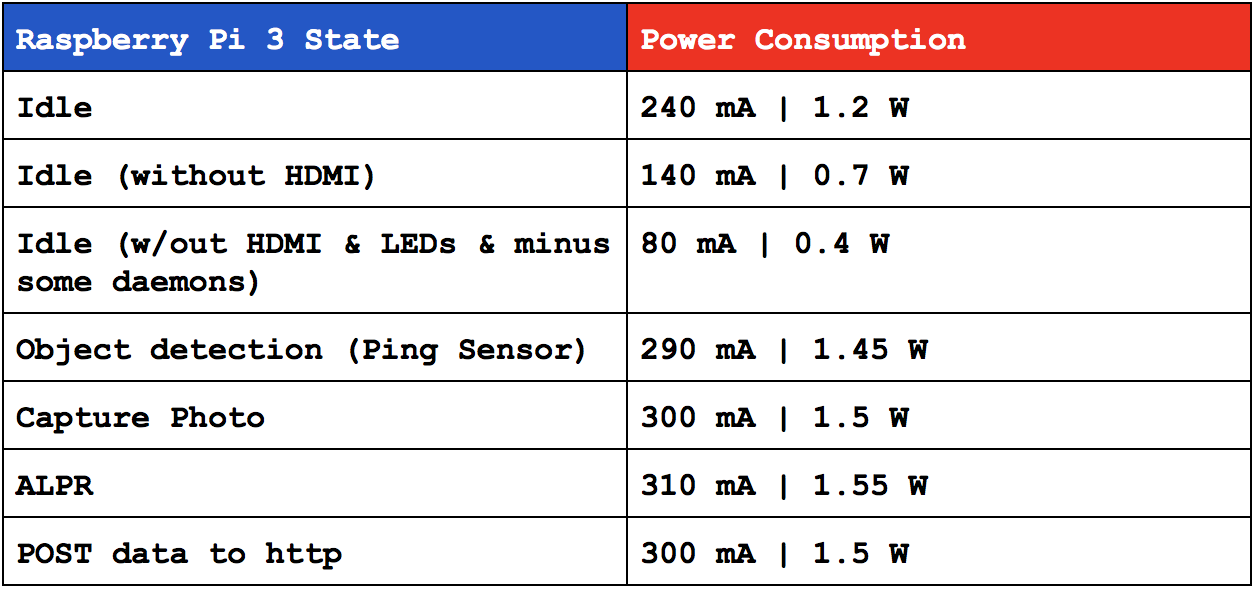
\includegraphics[width=0.9\textwidth]{pictures/Pipower.png}
\caption{This table shows the current power comsumption without the neopixel ring}
\end{figure}

As stated earlier in the document, power consumption was not the strong suit of this system. 
Given the table provided, we can immediately see the high current draws for idle states of the Raspberry Pi. 
When using high processing power with the image processing or communication to the database, we noticed a huge spike in energy consumption. 
When turning off the HDMI output port on the Pi, that took about 25 mA current draw off. 
By eliminating all the LEDs we brought our voltage down 5mA per LED. 
By disabling a few daemons on the Raspberry Pi  we got our current down by 100 mA or even more. 
We did not want to disable everything on the pi upon boot up. 
Overall we were able to limit the Raspberry Pi down to about 80 mA current draw which was about 0.4W.
In California, electricity averages around \$0.1534 kWh. 
Powering this sensor modules for an entire year for 24 hours a day would average you about \$0.53.

It was always in our knowledge to think of multiple directions we could optimize the energy consumption of each of our sensor modules.
Since SPOT is more of a system, we decided that energy consumption was by far the least of our worries and focus of the project.
In the future work discussion of this system document we will go into more detail about more viable solutions towards making our sensor modules optimal both with energy and functionality.
%%%%%%%%%%%%%%%%%%%%%%%%%
\subsection{Sensors}

\subsubsection{Proximity Sensing}
%%%%%%%%%%%%%%%%%%%%%%
\begin{figure}[ht!]
\centering
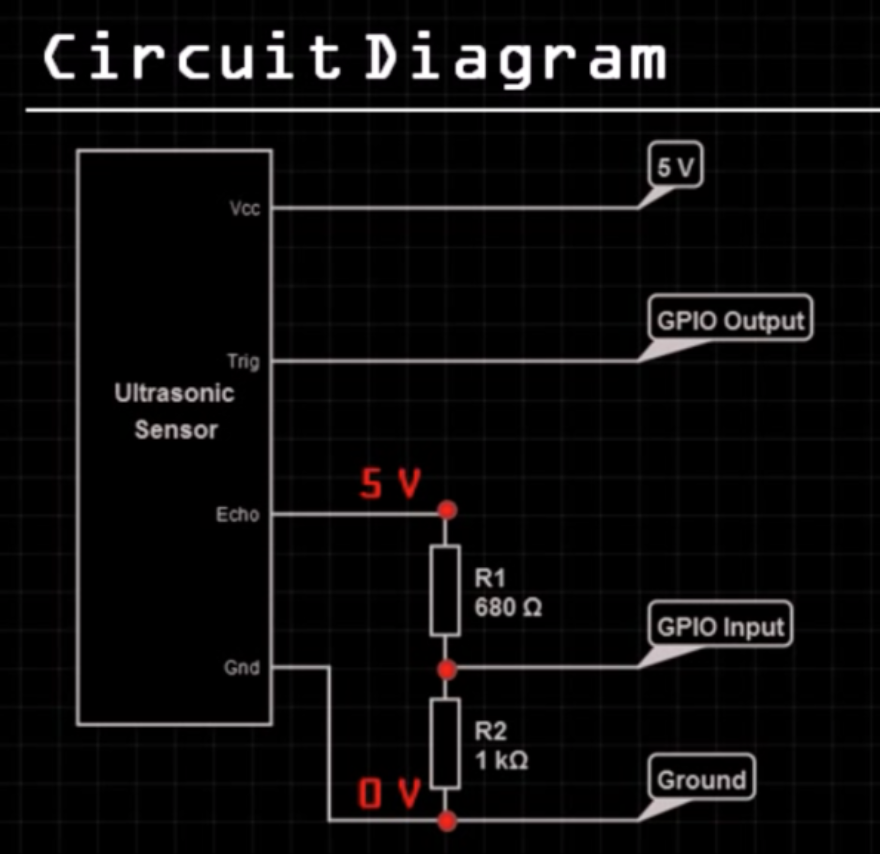
\includegraphics[width=0.5\textwidth]{pictures/ping_circuit.png}
\caption{This circuit shows our voltage drop across the echo to ground bringing the range from 0 to 5 volts down to around 0 to 3.3 volts into the GPIO input on our Raspberry Pi.}
\end{figure}
%%%%%%%%%%%%%%%%%%%%%
Our entire system and sensor module rely heavily on the sensors for proximity.
For our purposes, the ping sensor of our choice was the HC-SR04.
The data sheet can be found at from the link provided at the bottom. \footnote{https://cdn.sparkfun.com/datasheets/Sensors/Proximity/HCSR04.pdf}

This sensor is not always the best in terms of speed, but it can accurately give us distance in meters, feet, etc. 
This device is sequentially triggered causing the sensor to output sonic bursts that eventually return back to the device through the echo pulse output, hence the bit of delay causing the sensor to be a proximity tool. 
For our implementation we have the sensor connected through the GPIO pins on the Raspberry Pi through the circuit shown in Figure 4.
This voltage drop allows us to read precise measurements for the echo input into the Raspberry Pi. 
Since this ping sensor is extremely linear, round object detection does not always echo perfectly back.
The sensor is also on a time-based system, if the module does not hear back from the echo of the sonar pulse, it assumes there are no objects in front of it.
These two flaws are well known to us, but has not been proven to inhibit the ability of our proximity detection of a car pull into a SPOT.

Upon receiving the echo pulse output it returns a pulse width signal with the range in proportion.
This allows us to calculate the range through time intervals between sending a trigger signal and receiving an echo signal.

The reading conversion was quite simple:
\textit{
\begin{center}
    speed = $\frac{distance}{time}$
\end{center}
\begin{center}
         speed\ of\ sound = 340m/s = $\frac{2 \cdot distance}{time}$ 
\end{center}}
\begin{equation}
    distance = 170 m/s \cdot time
\end{equation}
%insert circuit design diagram

The python script we wrote functionally provides us with the ability to get accurate measurements for distances.

\begin{lstlisting}[language=Python]
while GPIO.input(ECHO)==0: # start timer 
  pulse_start = time.time()
while GPIO.input(ECHO)==1: # stop timer
  pulse_end = time.time()
pulse_duration = pulse_end - pulse_start
\end{lstlisting}

With the \textit{pulse\_duration}, we can easily use the time duration to calculate distance.
Upon initializing the Raspberry Pi for bumper detection in our file: \textit{bumper\_distance\_checker.py}, we set the GPIO pins for input and output.
Referring to the pinout from \ref{fig:rpi}, the pin we designated for \textit{GPIO.OUT} was 16 for the trigger output signal.

\begin{lstlisting}[language=Python]
GPIO.setup(TRIG,GPIO.OUT)
GPIO.setup(ECHO,GPIO.IN)
\end{lstlisting}
For the \textit{GPIO.IN} pin, we designated 18 for an input from the echo pulse response.
In the code, we set a short period of time, 1 milliseconds, allowing the ping sensor to settle then pulsed the trigger pin for a millisecond beginning the proximity process.

\begin{lstlisting}[language=Python]
GPIO.output(TRIG, True)
time.sleep(0.001)
GPIO.output(TRIG, False)
\end{lstlisting}

In the event if a person is simply crossing the sensor module, we trigger the sensor twice to make sure we get two very similar readings. 
If the error between the two proximity readings are above 10\%, we discard these results until the next period of measurements.
Once the two proximity measurements are accounted for and within the desired parking distance between the sensor module and the bumper, the sensor updates the local status file.
Once the Raspberry Pi is informed that there is an object in front via the status file, we continue to execute the rest of the automation script.

% Review this section
\subsubsection{License Plate Recognition}
Our system hopes to automate parking enforcement for our user. 
We leverage legally required licences plates, as a well instantiated form of visible ID, that can be used as a defense mechanism against unauthorized parking. Without camera-parsed license plate info, there’s no reliable way for our system to enforce appropriate parking. We’re currently using a well known algorithm OpenALPR to do all image processing for us right now. 
There's several dependencies to get OpenALPR running. OpenALPR directly depends on OpenCV and Tesseract, and Tesseract depends on Leptonica. All of these are image analysis frameworks required to get license plate recognition up and running.

Doing a pull from our github should give you all the setup script for openAlPR which install all dependencies. After everything should be ready to go! Depending on your drivers, you may need to update the camera driver to properly interface the OV5647 (RaspiCam). You can update to the appropriate driver using:

\vspace{0.5cm}
\begin{lstlisting}[language=bash]
$ sudo modprobe bcm2835-v4l2
\end{lstlisting}

With everything setup, you should be analyze a licencs plate using the following command:

\vspace{0.5cm}
\begin{lstlisting}[language=bash]
$ alpr check_myPlate.png 
\end{lstlisting}

This will return a list of license plate ID's and their associated probabilities. We use the most probable one.

\subsubsection{Status Light}
The status light is comprised of a Neopixel ring that is controlled by an Arduino Nano.
The Raspberry Pi controls the Arduino Nano through USB Serial communication. 
The necessary library can be easily installed by pressing \textit{Sketch \textgreater Include Library \textgreater Manage Libraries} and then:
\begin{verbatim}
#include <Adafruit_NeoPixel.h>
\end{verbatim}
The required setup on the Ardiuno files for serial communication requires:
\begin{lstlisting}[language=C]
Serial.begin(115200);
\end{lstlisting}
The Pi will send a 1 or a 0 if the ping sensor is triggered.
The Arduino Nano is programmed to only switch between the color green and red based on if the value from the Pi is 0 or 1. 
Upon connection the Ardiuno Nano is loaded with code that will iterate continuously.
If the serial is available for communication:
\begin{lstlisting}[language=C]
incomingByte = Serial.read() - '0';
if(incomingByte == 1) color(RED);
else if (incomingByte == 0) color(GREEN);
\end{lstlisting}
When a car is not occupying the SPOT, the Neopixel ring will default to green (0), which means not occupied.
When a car is in front of the SPOT, the Nexopixel ring will change to red (1), which will signify to the user that they are officially occupying the SPOT and billing will begin shortly. 
This UART connection is constantly running in the background so that the status light shown in \ref{fig:occupy} will change once the ping sensor triggers and notifies the cloud that there is a car.

\begin{figure}
\centering
\begin{subfigure}{.4\textwidth}
  \centering
  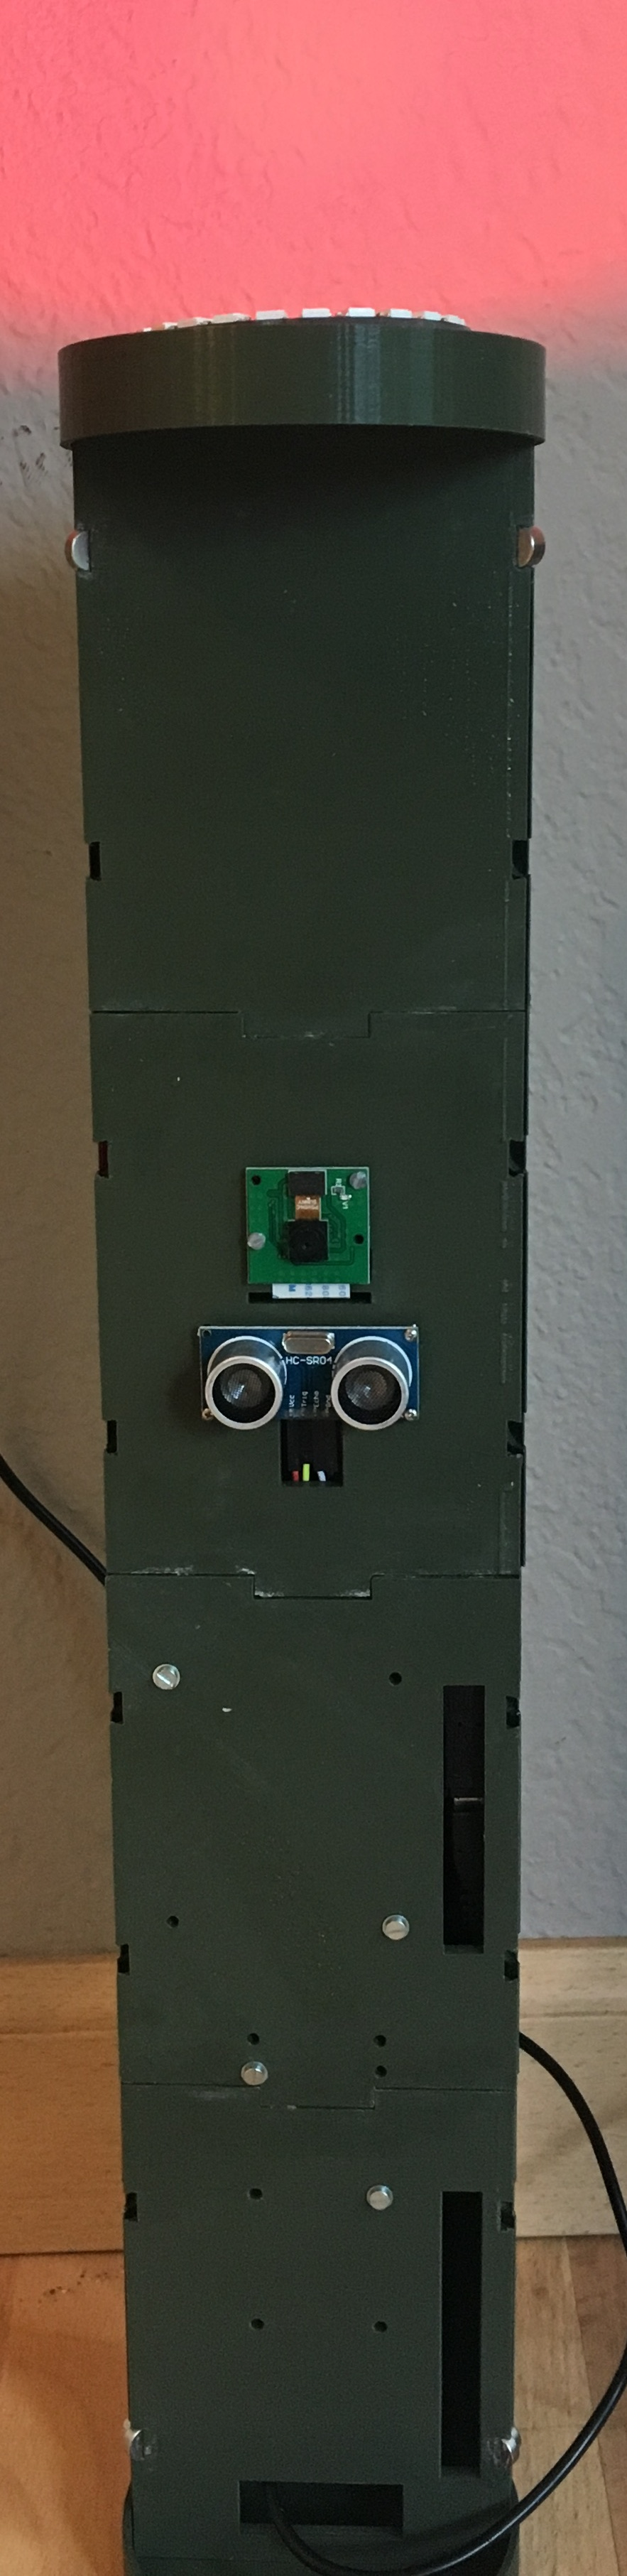
\includegraphics[width=.27\linewidth, height=8cm]{pictures/IMG_1664.JPG}
  \caption{SPOT with status: Occupied}
  \label{fig:3dprinted}
\end{subfigure}%
\hfill
\begin{subfigure}{.5\textwidth}
  \centering
  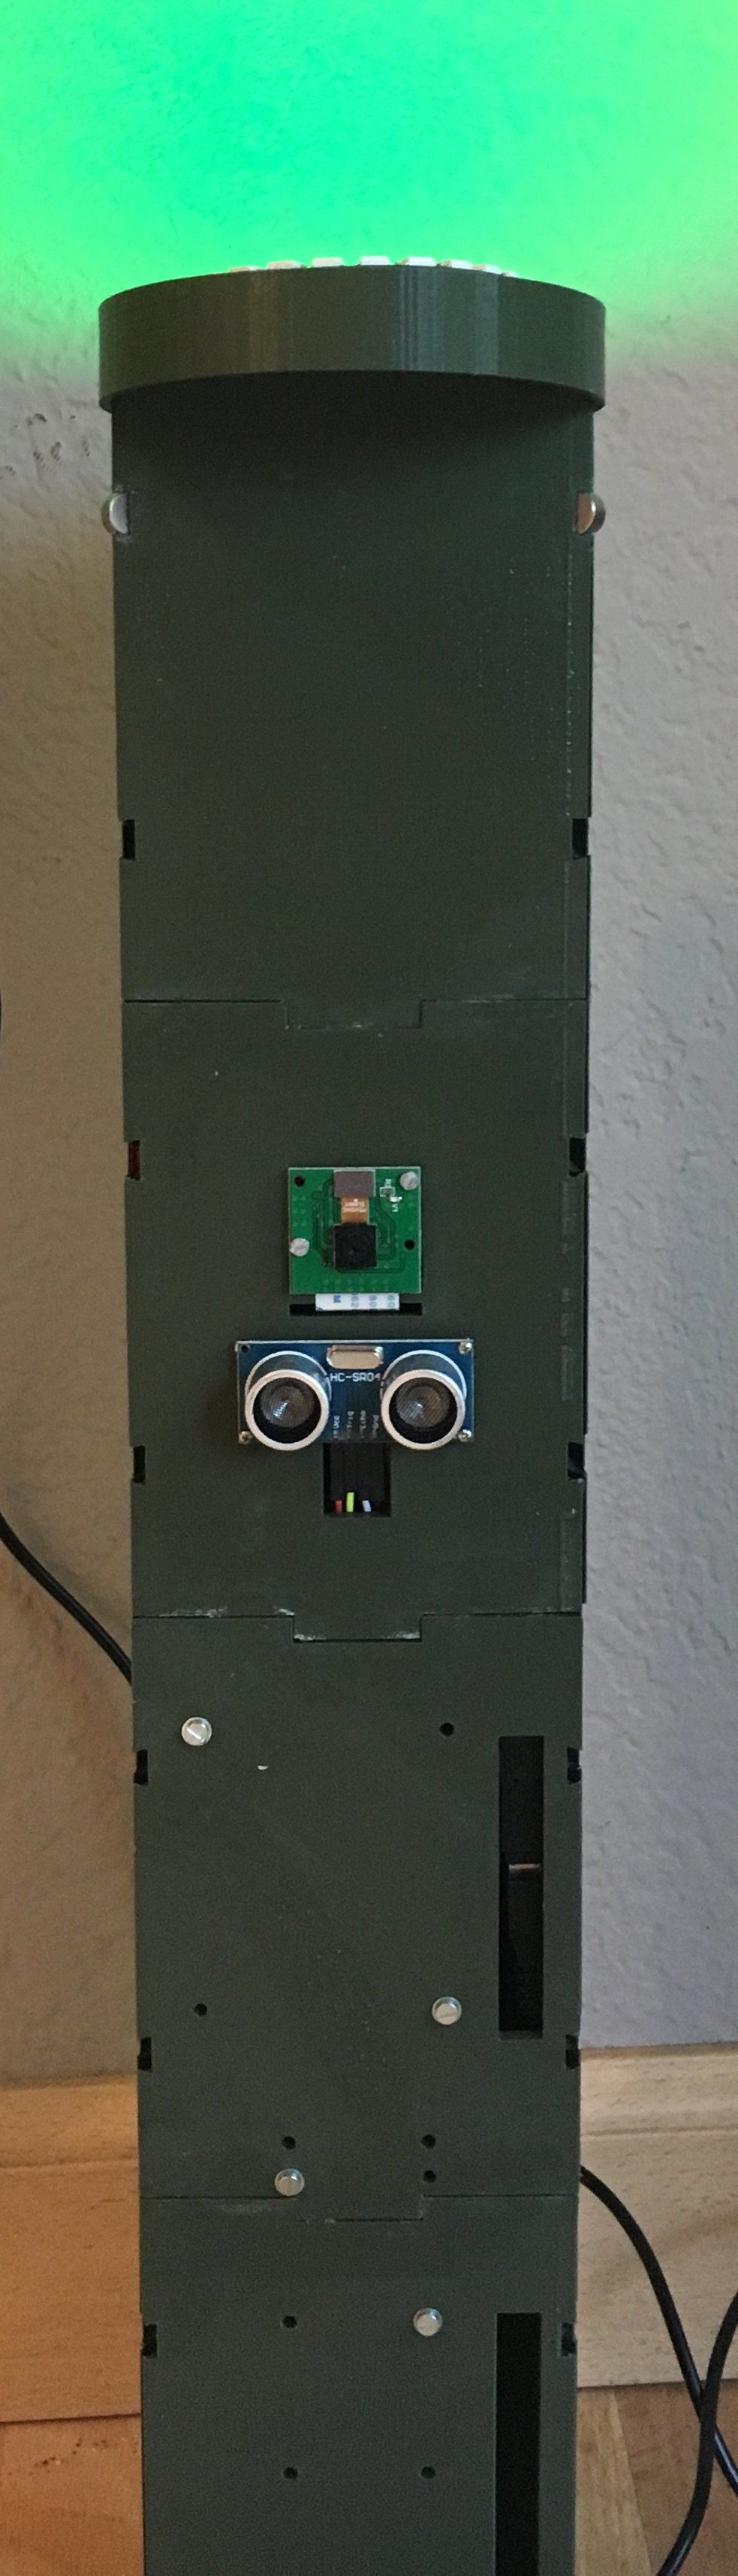
\includegraphics[width=.27\linewidth, height=8cm]{pictures/IMG_1668.JPG}
  \caption{SPOT with status: Unoccupied}
  \label{fig:acrylictube}
\end{subfigure}
\caption{Side By Side of Status Lights}
\label{fig:occupy}
\end{figure}

% \subsection{Future Implementations}%rephrase please, if you know a better one
%In here we can discuss other hardware & sensor options and briefly describe why we didn't use them or think these would be perfect from here on out
% Shouldn't we just be doing this in the future_work section?
